\documentclass[british,titlepage]{ntnuthesis}
\raggedbottom
\usepackage{graphicx}
\usepackage{caption}
\usepackage{adjustbox}
\usepackage{biblatex}
\usepackage{placeins}
\usepackage{gensymb}
\usepackage{algorithm}
\usepackage{float}
\usepackage{glossaries}
\usepackage{algpseudocode}
\usepackage{listings}
\lstset{language=Python,
    basicstyle=\fontsize{9}{12}\ttfamily,
    keywordstyle=\color{blue}\ttfamily,
    stringstyle=\color{red}\ttfamily,
    commentstyle=\color{olive}\ttfamily,
    morecomment=[l][\color{magenta}]{\#},
    showstringspaces=false,
    breaklines=true,
    frame=tb
}
\usepackage[most]{tcolorbox}
\usepackage{multirow}
\usepackage{appendix}
\usepackage{spverbatim}
\setcounter{secnumdepth}{3}
\graphicspath{ {chapters/figures/} }

\title{Private Information Inference Based on Network Traffic Patterns of AQMs}
\author{H. Knudsen}
\date{01.06.2023}
\pagenumbering{roman}
\addbibresource{thesis.bib}


\makeglossaries

% --------------------
% ----- Acronyms -----
% --------------------

\newacronym{IoT}{IoT}{Internet of Things}
\newacronym{RQ}{RQ}{Research Questions}
\newacronym{Wi-Fi}{Wi-Fi}{Wireless Fidelity}
\newacronym{SSID}{SSID}{Service Set Identifier}
\newacronym{AQM}{AQM}{Air Quality Monitor}
\newacronym{VOC}{VOC}{Volatile Organic Compounds}
\newacronym{LAN}{LAN}{Local Area Network}
\newacronym{AP}{AP}{Access Point}
\newacronym{BSS}{BSS}{Basic Service Set}
\newacronym{ISP}{ISP}{Internet Service Provider}
\newacronym{CRC}{CRC}{Cyclic Redundancy Check}
\newacronym{WEP}{WEP}{Wired Equivalent Privacy}
\newacronym{WPA}{WPA}{Wi-Fi Protected Access}
\newacronym{pcaps}{pcaps}{Packet Capturings}
\newacronym{pkt}{pkt}{packet}
\newacronym{SD}{SD}{Standard Deviation}
\newacronym{MAC}{MAC}{Media Access Control}
\newacronym{TVOC}{TVOC}{Total Volatile Organic Compounds}
\newacronym{VS Code}{VS Code}{Visual Studios Code}
\newacronym{DNS}{DNS}{Domain Name Service}
\newacronym{TCP}{TCP}{Transmission Control Protocol}
\newacronym{UDP}{UDP}{User Datagram Protocol}
\newacronym{ICMP}{ICMP}{Internet Control Message Protocol}
\newacronym{HTTPS}{HTTPS}{Hypertext Transfer Protocol Secure} % add glossary and acronym lists before document

\begin{document}
\textbf{Title:}\hspace{2cm} Private Information inference in air quality monitors
\\\\
\textbf{Student:}\hspace{2cm} Helene Skjelsbæk Knudsen
\\\\\\
\textbf{Problem Description:}\\
Internet of Things are becoming more widespread and more available for any user. Devices that normally did not communicate with other devices, are being given functionality by adding sensors and technology. This functionality can be used to communicate with other devices, servers on the cloud or make their decisions. Producers of these devices are constantly adding functionality and new devices to keep up with the increasing demand from users wanting to create smart homes. Turning on the heat at your home from another location through an application on your mobile phone or having the doorlock send you notifications when it is opened or locked are examples of functionality that makes up the Internet of Things.
\\\\
Air Quality Monitors are a type of Internet of Things devices that monitors the indoor climate in any users home. The devices can communicate over different communication protocols to their apps or the vendors cloud storage. In addition, their functionality varies as they as equipped with different sensors giving the users different values of how good or bad their indoor climate is. The monitors can communicate with other devices and be integrated in a smart home environment. However, having devices monitoring your home 24/7 arises security issues. Private information about user behaviour can be attractive to different parties, from company's wanting to know how to target advertises to malicious actors that wants to misuse the knowledge of users habits. 
\\\\
This thesis will investigate several different Air Quality Monitors to see how and what private information can be gathered from carrying out a passive network eavesdropping attack. As the market contains a wide variety of air quality monitor devices, a few devices from different vendors should be chosen to carry out the attack and discovery what kind of private information in a user environment can be collected. 
\\
\ \\
\begin{flalign*}
     \\\textbf{Supervisor:}&& \text{Jia-Chun Lin, NTNU}
\end{flalign*}
\chapter*{Abstract}
The emerging use of IoT devices in homes arises security concerns whether or not these devices expose private information about users and their environment. Air quality monitors are a type of IoT devices which are always on to monitor the indoor air quality of the environment. Even though air quality monitors have been included in several tests within security, there are research gaps in comparing different devices to each other and conducting test cases specifically designed to see if there are differences in the level of inference on the air quality monitors. This master thesis carries out a passive network eavesdropping attack on three different air quality monitors to investigate if the network traffic pattern changes during a triggered event and if these patterns can be used to infer user activities. The devices all communicate over Wi-Fi and are manufactured from different vendors. The research first presents with a baseline capture of the devices to learn their traffic patterns when events are not triggered. Then four different test cases were tested on the devices to see if it is possible to infer private information through looking at the corresponding network patterns. The test cases designed in this thesis are cooking, showering, window open during night, and weekends at home or gone. The results showed that only one of the air quality monitors expose private information from one of the test cases. For this device it is possible to infer whether a user is home or gone by looking at bytes sent and received and the differences in packet sizes. This private information can be misused by an adversary to know when a user is home or not just by looking at the Wi-Fi traffic sent to and from that device. This research demonstrates that air quality monitors communicating over the same protocol, in this case Wi-Fi, have different traffic patterns and expose private information differently. It also motivates to continue the research on air quality monitors, as these have not been as popular to test as other IoT devices. 
\chapter*{Sammendrag}
Den økende bruken av IoT enheter i hjem skaper sikkerhetsutfordringer med tanke på om disse enhetene avslører privat informasjon om brukere og hjemmemiljøet. Luftkvalitetsmålere er en type IoT
enheter som alltid er påskrudd for å måle den luftkvaliteten innendørs. Selv om luftkvalitetsmålere har vært inkludert i flere sikkerhetstester, er det mangler i forskningen på å sammenligne ulike enheter med hverandre og å utføre tester som er spesifkt designed for å se om det er forskjeller i hvor mye privat informasjon enhetene avslører. Denne masteroppgaven utfører et passivt nettverksavlytnings angrep mot tre ulike luftkvalitetsmålere for å undersøke om mønstre på nettverkstrafikken endrer seg når en test utføres og om dette kan brukes for å hente ut privat informasjon for å fange opp brukeraktivitet. Alle enhetene kommuniserer over Wi-Fi og er laget av ulike produsenter. Oppgaven presenterer først standard trafikk fra enhetene for å se på mønstre på nettverkstrafikken når det ikke blir utført spesfikke tester i miljøet. Deretter, ble fire ulike tester utført i miljøet til enhetene for å se om det var mulig å hente ut informasjon om miljøet ved å se på tilsvarende nettverksmønstre. De fire testene som ble utført er lage mat, dusje, ha vindu åpent på natten og helg hjemme eller borte. Resultatene viste at kun en av luftkvalitetsmålerne avslører privat informasjon fra en av testene utført. Fra trafikken på denne enheten er det mulig å se om en bruker er hjemme eller ikke ved å se på bytes sent og mottatt og forskjeller i pakkestørrelse. Denne informasjonen kan bli misbrukt av en ondsinnet aktør ved å vite om brukeren er hjemme kun ved å se på trafikken sendt over Wi-Fi, til og fra enheten. Testene viser også at ulike luftkvalitetsmålere som kommuniserer med samme protokoll, i denne sammenheng Wi-Fi, har ulike mønstre på nettverkstrafikken og avslører privat informasjon ulikt. Dette motiverer også til å fortsette testingen på luftkvalitetsmålere, siden disse ikke har vært like populære å teste som andre IoT enheter. 
\chapter*{Preface}
This document serves as my Master Thesis in Information Security and concludes my 3-year degree at the Norwegian University of Science and Technology, NTNU, department Gjøvik.
\\\\
I would like to thank my supervisor, Jia-Chun Lin, for being a great support and challenging me to learn new things during my writing process. I would also like to thank everyone in our \gls{IoT}group; Benjamin Ulsmåg, Mathias Hedberg, Kevin Nordnes, Lloyd Nicolay Gustavsson, Aafan Ahmad Toor, Ming Chang Lee and Ernst Gunnar Gran for sharing their knowledge and being discussion partners througout this project. 
\\\\
At last, I would like to thank my partner Benjamin for supporting me in all phases of the thesis. I could not have done it without you. 
\\\\\\
Helene Skjelsbæk Knudsen, 01.06.2023


\tableofcontents
\listoffigures
\listoftables

\printglossaries
\printglossary[type=\acronymtype] 

\pagenumbering{arabic}
\chapter{Introduction}
This chapter introduces the master thesis while presenting the background and motivation, followed by the research objectives and research questions that will be answered throughout this research. Scope and delimitation gives a clear understanding of what is included and not included in the thesis. While the thesis structure outlines and gives a brief understanding of each of the following chapters in this thesis. The contribution that this thesis aims to give to research are presented in a separate subsection. 

\section{Background and motivation}
The Internet of Things (IoT) exists of a growing number of physical devices connected to the Internet to perform smart tasks \cite{IoTSurveyAl-Fuqaha}. Every-day devices can be equipped with smart functionality to improve our lives, but also to improve critical societal functions such as in health care or industrial technology. The devices can range from a robot vacuum cleaner that users can control through their phone or cameras installed for elders to stream to a nurse who resides centrally. These smart devices can communicate and connect to each other and other services using the Internet and makes out an IoT system. The devices analyzes how users, machines or eco-systems behave and act accordingly. An emerging request for smart devices has resulted in an rapid growth in IoT devices worldwide \cite{IoTAndPrivacy}. The devices are becoming more user friendly, smarter with added functionality and aesthetically more suitable to place or wear in any environment. 
\\\\
We spend a lot of our lives inside, breathing in the air that is available in the indoor space \cite{IndoorAirQualityMonitorIoT}. The air affects our health and can potentially cause several chronic health problems, for example lung cancer or respiratory infections \cite{IAQMonitorReview}. Common air pollution's, such as smoke or car exhaust, are easy to sense and avoid for people not trying to get effected by the dangerous particles they emit. It is also more wide-known that good outdoor air is beneficial for your health, not considering that the air indoor can also severely affect your health \cite{IndoorAirQuality}. Therefore, including the fact that Internet of Things devices are evolving, indoor air quality monitors are increasing in popularity and functionality \cite{SecurityAndDataIntInAQM}. The air quality monitors are also developing into becoming smaller, more affordable and appealing to include in your home environment while adopting several different sensors to report on the indoor air quality trying to become a more popular choice for users. 
\\\\
As users are installing these sensors inside their own homes and allow them to monitor their home environment every single day, they will be collecting data about the environment and changes or behaviour that affect the air quality monitor sensors. Therefore,it is interesting to look further into how easy it is to collect this data and infer what kind of user behaviour is happening in the environment. As harmless as a passive sensor, that is just collecting data about different indoor climate rates may seem, it is important to understand the risks one takes when installing these and connecting them to the Internet. Understanding what kind of private information is possible to infer from these devices and what makes the differences can be crucial when deciding which air quality monitor on the market to buy and install in your home.

\section{Research Objectives and Research Questions}
This thesis will conduct a network attack called passive network eavesdropping attack, that will be further explained in the background and method, and launch it against a group of individual air quality monitors residing in a home environment. In order to decided which devices to use and how to carry out an attack, a survey of the devices will be presented. A justification for which test cases to engage the sensors and devices is important when analyzing the results. When the network eavesdropping attack have been carried out and data  from the different test cases are collected the results will be analyzed to see if and how much private information can be gathered from the different devices. The results will also look into if there are significant differences between the air quality monitors. Lastly, the research will investigate how the private information inferred can be used by malicious actors in a harmful way for users having the air quality monitors installed in their home.
\\\\
Based on the problem description, motivation and research objectives, the following research questions (RQs) have been raised and will be answered throughout the research of this master:
\begin{itemize}
    \item 
    \textbf{RQ1:} What kind of information can be gathered from air quality monitors when carrying out a network eavesdropping attack? And what kind of private information about the users and the environment can be inferred from the collected traffic?\\
    \item 
    \textbf{RQ2:} What are the differences in level of inference from different air quality monitors from different vendors?\\
    \item 
    \textbf{RQ3:} How can the private information gathered be misused by an adversary?\\
\end{itemize}

\section{Research Scope and Delimitation}
This research presents 3 different air quality monitors, all selected from different vendors. The air quality monitors communicates over the same protocol, Wi-Fi, but have different functionalities, applications and sensors. A Wi-Fi sniffer together with \textit{tshark} running on \textit{Kali Linux} will be used to sniff and store traffic from the sensors. To be able to answer the research questions, a baseline traffic pattern will be compared to traffic during triggered scheduled user events. The goal is to investigate what kind of private information, if any, it is possible to collect from conducting a passive network eavesdropping attack on the different devices and give an understanding of how this information can be misused if an adversary gains access. 
\\\\
This thesis will not look into decrypting traffic if the air quality monitors encrypt the communication. The focus will be on conducting a passive network privacy inference attack and therefore only look at non-encrypted data whether it is the whole packet or only the header. The research will also not look into different factors of how to do a successful attack, such as distance, materials of the building or power of the sniffer. The thesis will not cover all phases of a passive network eavesdropping attack, but a prerequisite of this is that the attacker has gained a strong enough wireless access to the users network through their Service Set Identifier (SSID) to be able to read traffic sent from and to the devices in the environment. It will not look into how to identify the IoT devices as they are already known with MAC address in this research. However, there are a numerous of researches that have looked into identification of several different IoT devices, such as \cite{IdentifyIoT1} and \cite{IdentifyingIoT2}. 

\section{Contribution}
This thesis contributes with research on different individual air quality monitors and what kind of private information that can be inferred from them. Even though there are other researches that have carried out a passive network eavesdropping attack trying to infer private information from IoT devices, a lot of these researches investigate on IoT devices that can clearly pose a threat to users privacy if inferred, such as cameras, watches or motion sensors. In a lot of researches found online, air quality monitors are often a part of an IoT environment and only one type of air quality monitor are included in the same environment, making it harder to compare the differences between different brands and sensors. Research on specifically air quality monitors are popular when it comes to their functionality and sensor and how good they can read the indoor environment, but looking into security and privacy of the devices, the research decreases significantly. Therefore, will this research contribute to not only looking into if a passive network eavesdropping attack can expose private information, but also if there are differences when multiple indoor air quality monitors are placed to observe the same environment and are exposed to the exact same test cases. 

\section{Thesis Structure}
This thesis is structured in the following chapters:\\\\
\textbf{Background}
\\
The background defines and describes important information for the reader to be able to understand the research and results. The background first presents general information about air quality monitors, how they work, how the sensors works and what factors plays a part when selecting which air quality monitor to buy. The concepts of private information inference and passive network eavesdropping are explained as these are the method that will be used on the devices to answer the research questions. Lastly, Wi-Fi is explained and elaborated as this is the communication protocol that the devices communicate over and where the sniffing will take place. 
\\\\
\textbf{Related Work}
\\
The related work chapter aims to give the reader a selection of previous work and published research done by others on the topic. Former research on the security and privacy issues of specifically air quality monitors have the largest weight in this chapter. Both attacks, security frameworks and suggestions and privacy challenges are included in this section. As air quality monitors are a part of IoT devices, the other section of this chapter highlights research done on misusing of private information on IoT devices, where research done on IoT devices in general or a smart home or smart home care environment with several different IoT devices. 
\\\\
\textbf{Method}
\\
The method will describe in detail how this research has been carried out and give justification on the choices made. The survey for choosing the air quality monitors are presented and a more detailed description on the three devices chosen and how they work are presented. To ensure reputability, the environment setup are shown for both hardware and software components used to carry out the attack. Lastly, the test cases closes up the chapter by giving justification on why they were specifically chosen and how they are designed and details on how they are carried out. 
\\\\
\textbf{Evaluation and Analysis}
\\
\\\\
\textbf{Discussion}
\\
Fallgruver!! Hva kunne jeg gjort bedre?
\\\\
\textbf{Conclusion}
\\
The conclusion will conlude this research by answering the research question in short term and summing up this master thesis. 
\chapter{Background}
This chapter gives an overview of the necessary background information required for this research. Air quality monitors are explained in a general way with its use, capabilities and sensors. Passive network eavesdropping and private information inference are introduced as this will be the vulnerability exploit in this research. Lastly, this chapter gives an overview of Wi-Fi, Bluetooth, ZigBee and Ethernet that are communication protocols which air quality monitors use to communicate over. \\\\
\section{Air Quality Monitors}
Air quality monitors are used as sensors to collect sensor data from different sources in the air. \cite{GeneralAirQualityMonitor} The IoT devices can store data in different ways. Cloud storing is the most preferred storage solution for IoT devices, but also local servers, internal storage and SD cards can be used to store data from IoT devices and air quality monitors. \cite{AQMBigSource} Displaying data to users of air quality monitors is an important factor to give the user either just information about the indoor quality, or recommendations on how to better the air. \cite{AQMBigSource} The most developed and recent method of doing so, is through an app on the users mobile phone, but also solutions where users can login to a web-site exists. Many air quality monitors also have the functionality of an screen on the device that shows certain values from the sensors. Some of these can also be interactive. \cite{AQMBigSource}
\\\\
Several factors plays a key part when selecting which air quality monitor most suitable for the users needs. Even tough many devices are pre-calibrated when available in store, a test on the specific environment should be done. Considering the different functionality an air quality monitor can have, it is also important to look into transmission range, power consumption and requirements for maintenance. \cite{AQMBigSource} However, the main goal of an air quality monitor is to monitor the air and therefore looking into which kind of sensors the devices have should be a top priority when selecting your device. Air quality monitors can specialize in one measuring unit in the air or have the functionality to measure several air quality factors, such as \(CO_2\), radon, HCHO, noise, VOC, humidity or temperature. The air quality monitors are incorporated in users homes and therefore the appearance of the device will also be a considerable factor for choosing the right device. \cite{IAQMonitorCommunicationReview} 
\\\\
As indoor air quality monitors can be equipped with different features, a brief explanation of some of the features an air quality monitor can sensor is necessary to understand why and how private information can be gathered from these sensors:
\begin{itemize}
    \item \(CO_2\)\\
        Carbon Dioxide, \(CO_2\), is a chemical formula that is made by human or animal combustion, in addition to other larger combustion processes. \cite{CO2} This implicates that the more humans or animals that are in the same indoor environment as the air quality monitor, the higher occurrence of \(CO_2\) will be collected by the sensor and transmitted to the air quality monitors receiver. However, plants and sunlight can bind \(CO_2\) and reduce the amount of \(CO_2\) particles in an indoor environment. Also bad or irregular ventilation will make the \(CO_2\) levels grow.
    \item Radon\\
        Radon is a radioactive gas that is strongly recommended to be measured in Norwegian indoor environments. \cite{Radon} The gas does not have any smell and is invisible and is carcinogenic which makes it an attractive feature to include on the air quality monitor. 
    \item Noise\\
        Noise is an interesting feature of some air quality monitors as it considered a health problem. \cite{Noise} Exposure to loud noises at a small amount of time or long-term noise can both harm peoples health. Especially when considering a work environment where workers need to concentrate, noises over long periods of time can result in hearing difficulties or problems communicating. As many work from home and we use a lot of time in our home, the problem is also applicable here. 
    \item VOC\\
        Volatile organic compounds, VOC, is a collective term for any combination of carbon, with the exception of carbon monoxide, carbon dioxide, carbonic acid, metallic carbides or carbonates and ammonium carbonate. \cite{VOC} These harmful compounds can be found in gases from building materials or smoking, cleaning articles, painting or cooking to mention some. TVOC is a term for defining the total amount of VOCs. The amount of VOC in the indoor environment can be simply reduced by ensuring fresh air and using kitchen fans to prevent the articles from circulating the indoor air to be breathed by users. \cite{RecommendedIAQ}
     \item HCHO\\
        HCHO is the chemical formula for formaldehyde which is a gas that can cause severe health effects. \cite{HCHO} The gas contains a strong odor and is flammable when it has room temperature, but is colorless. People can be exposed to HCHO from several different sources such as manufacture wood products, building materials, fertilizers, cigarettes, paint, glue or even medicines and cosmetics. Formaldehyde is classified as a VOC.
    \item Humidity\\
        Humidity is calculated from the ratio between water vapor in the air compared to the maximum amount of water vapor possible in the air if the air was saturated. \cite{RecommendedIAQ} Even tough humans can endure high variations in humidity, very low percentages of humidity can result in health problems such as irritated eyes, dry skin or dry moucus membranes. The humidity is correlated by temperature, which means that variations in temperature can effect the humidity percentage. Normal home behaviour that can affect the humidity is taking a shower, drying clothes and cooking. 
    \item Temperature\\
        Temperature is a measure unit for how hot or cold the environment is and is measured using a thermometer. Temperature is the most commonly used unit for how comfortable humans feel. Temperature can affect humans health on both ends of the scale. A too high temperature can result in lack of energy and sleepiness and a too low temperature can result in reduced muscle function or heighten symptoms of rheumatism. \cite{Temp}
\end{itemize}


\\\\
As air quality monitors can be a part of a smart home care system, it can also include in a Wireless Body Area Network (WBAN) to sensor the indoor environment. Therefore, it can be vulnerable to several security threats and attacks by malicious actors. \cite{AttackstoAQMs} 
\\\\

\subsection{Private Information Inference}
Considering the amount of information an air quality monitor can collect about an individual or a smart home, privacy leakage is a vulnerability. \cite{SecPrivSmartCity} When malicious attackers tries to gather sensitive information about an individual user or group of users, a privacy attack is carried out. \cite{CyberEntitySecInIoT} The aim of the attacker is then to target the confidentiality of the user, while gathering information such as location, preferences, personal behaviour or similar private information.

\subsection{Passive Network Eavesdropping}
Eavesdropping network communication can either be passive or active. When an attacker conducts an active eavesdropping attack on a target, the data in the communication link is both inferred and modified. \cite{Eavesdropping} While in a passive network eavesdropping attack, the eavesdropper does not modify any data on the link, but simply aims to gather data transmitted without changing the communication. The overall goal of eavesdropping is therefore often to access private information that are being sent on the channel. That can be anything from credentials to secret messages, or as in this research, private information about users and their habits. \cite{Eavesdropping} Since the communication is not effected by a passive network eavesdropping attack, the attacker does not need to be as careful in disguising itself as in an active attack.  
\\
There are security measures to implement to reduce the chance of being eavesdropped, both actively and passively. Since an eavesdroppers goal is to listen in on the communication, encrypting the traffic is an effective way to make it harder to conduct an eavesdropping attack. Also, covert channels that hide the identity of the communicating parties can be used to prevent the eavesdropper from finding the right communication channel to eavesdrop. \cite{Eavesdropping}
\\\\
\section{Communication Protocols}
Air Quality Monitors send their sensoring data to remote server for storing and analyzing the data. As they exists with different functionality and specifications, their communication protocols differs, like other groups of IoT devices. \cite{AQMBigSource} Wi-Fi is the most preferred protocol with Bluetooth and Zigbee following. \cite{saini2020indoor} As this thesis is delimited to air quality monitor devices that uses Wi-Fi, Bluetooth, Zigbee or wired communication trough Ethernet as communication protocols, the next subsections will elaborate on these protocols and specifications to be used further in this thesis through testing and analysis. 

\subsection{IEEE 802.11 - Wi-Fi}
Wireless Fidelity (Wi-Fi) \cite{WiFiAlliance} is one of the worlds most used technology for communicating and is defined, developed and standarized by WiFi Alliance. \cite{WiFiAlliance} Wi-Fi is based on the standard IEEE 802.11 Wireless LAN set by IEEE Standard for Information Technology. \cite{WifiStandard} The transmission range for Wi-Fi is up to 100 meters and it uses 5-60GHz in the frequency band. \cite{IAQMonitorCommunicationReview}
\\\\

\\\\
\subsection{Bluetooth}
Bluetooth is a communication protocol based on the IEEE 802.15.1 standard set out by the IEEE Standard for Information Technology. The frequency band for Bluetooth is 2.4GHz and the transmission rate is up to 10 meters, which is relatively shorter compared to Wi-Fi. \cite{IAQMonitorCommunicationReview} Due to the transmission range of Bluetooth it is mainly used for short-range communication, which can be very suitable for air quality monitors configured to transmit data to a hub or nearby other wireless devices, such as mobile phones. Since many IoT devices are designed to communicate in short ranges within a house, Bluetooth Low Energy (BLE) was introduced as a version suitable for this specific communication. \cite{SecurityofCommunicationProt} As the name says, BLE has a reduced power consumption, compared to WiFi, and is therefore often chosen as communication protocol for IoT devices. 
\\\\
When a Bluetooth device are starting a data exchange with another device, a paring process is established between the two communicating parties \cite{BluetoothCommunication}. The parties are one slave and one master, where the master is usually the device with the highest resources. For example an IoT devices, such as AQMs, as slaves and mobile phones as master. They find each other by listening to an advertising channel where devices waiting to connect are broadcasting messages. When connected, the parties change to another channel to exchange data called a Piconet. This channel is divided into time-slots where each party has its slots for communicating. The channel has the masters MAC address as the piconet address. This functionality makes it harder to eavesdrop as communication is not demand-based, but based on time slots. 

Bluetooth packets contains the following fields, also shown in figure X

\begin{itemize}
    \item \textbf{Channel Access Code:} Identifies the communication on the specific physical channel. 
    \item \textbf{Packet Header:} Includes source and destination for the packet and are used to route the packet. Also includes link control protocol. 
    \item \textbf{Guard and Sync:} Only used for enhanced data rate packets where guard time and synchronization is necessary before the payload is examined.
    \item \textbf{Payload Header:} Includes logic link identifier used for further routing and the size of the following payload.
    \item \textbf{Payload Body:} The field where the actual data transmitted relies. 
    \item \textbf{Message Integrity Check:} Only used with AES-CCM encryption.
    \item \textbf{Cyclic Redundancy Check:} Detects if packets have errors. 
\end{itemize}


\subsection{ZigBee}
ZigBee is also a popular choice for communication protocol when it comes to IoT devices. The protocol is based on the IEEE 802.15.4 standard set by IEEE Standard for Information Technology, but is developed by the Zigbee alliance \cite{ZigBeeStandard} \cite{ZigbeeAlliance}. ZigBee uses the same frequency band as Bluetooth, 2.4GHz, but also supports the frequencies 915MHz and 868MHz, and does obtain a longer transmission rate up to 20 meters. \cite{IAQMonitorCommunicationReview} The 2,4GHz frequency band contains 16 different channels for communication. \cite{ZigbeeOverview} Some of the advantages of ZigBee, and especially in IoT devices, are low data rate, low cost and long battery life. 
\\\\
ZigBee MAC-frame consists of three main parts, header, payload and footer, and four header fields, see figure \ref{ZigBeePic} \cite{ZigBeBasics}:
\begin{itemize}
    \item \textbf{Frame Control:} Contains information about the frame type, addressing fields and additional control flags.
    \item \textbf{Sequence Number:} Beacon Sequence Number
    \item \textbf{Addressing Fields:} Addresses for source and destination
    \item \textbf{Auxiliary Security HDR:} Optional and used for security processing
    \item \textbf{MAC Payload:}  The payload of the frame
    \item \textbf{MAC Footer (MFR):} Data verification with frame check sequence
\end{itemize}

\begin{figure}[h]
    \centering
    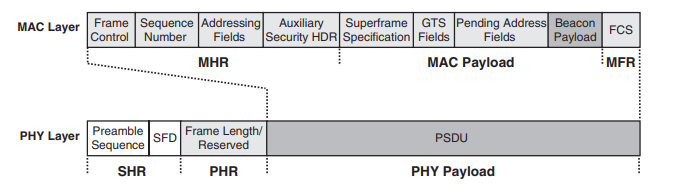
\includegraphics[width=0.5\textwidth]{figures/Zigbee.png}
    \caption{ZigBee MAC frame}
    \label{ZigbeePic}
\end{figure}

\subsection{Ethernet}

\subsection{Comparison of the different communication protocols}
In Table \ref{CommunicationProtocolsComparison} a comparison of the different communication protocols that will be used during tests in this thesis and their specifications are presented. \\
\begin{table}[!hbtp]
\begin{tabular}{||c | c | c | c ||} 
 \hline
 Communication Protocol & Frequency Band & Transmission Range & Power consumption\\ [0.5ex]
 \hline\hline
 Wi-Fi & 5-60GHz & 100m & High\\ 
 Bluetooth & 2.4GHz & 10m & Low\\
 ZigBee & 2.4GHz & 20m & Low \\
 Ethernet & Very variable & 100m & Plugged\\ [1ex] 
 \hline
\end{tabular}
\caption{Communication Protocols Comparison}
\label{CommunicationProtocolsComparison}
\end{table}
\chapter*{Related Work}

\subsection*{\textbf{RQ1}}
\addcontentsline{toc}{section}{RQ1}
\textit{What kind of private information can be gathered from air quality monitors when carrying out a network eavesdropping attack?}
\\\\
Related work\\\\

\subsection*{\textbf{RQ2}}
\addcontentsline{toc}{section}{RQ2}
\textit{What are the differences in level of inference from different air quality monitors from different vendors?}
\\\\
Related work\\\\

\subsection*{\textbf{RQ3}}
\addcontentsline{toc}{section}{RQ3}
\textit{What are the differences in level of inference from network eavesdropping air quality monitors communication on different protocols?}
\\\\
Related work\\\\

\subsection*{\textbf{RQ4}}
\addcontentsline{toc}{section}{RQ4}
\textit{How can the private information gathered be misused by an adversary?}
\\\\
Related work\\\\
\chapter{Method}
This chapter describes the material and method for testing, the environment setup and the test cases that has been conducted. First, a survey for selecting the air quality monitors that will be used in this research are introduced. Then, the method for creating the environment, carrying out the tests, and analyzing the results are presented in a method three and explained in details.  

\section{Air Quality Monitor Survey}
To select the air quality monitor to use in this thesis, the problem description and research questions have been used as a reference. In order to answer the RQs, the air quality monitors needs to be manufactured from different vendors. To find the specific \gls{AQM}s to use in this research, several online sources were used and compared. As this research is conducted on NTNU Gjøvik in Norway, it is also preferable that the devices are bought and available in Norwegian stores or online pages. The devices chosen should also be popular and easy accessible for any user. 

It exists many solutions that integrate air quality monitors within other devices, but as this thesis aims to investigate what private information are possible to infer from an air quality monitor, the devices should only have air quality monitoring functionality.  Considering these factors, the following criteria are made out to select the devices:
\begin{itemize}
    \item The devices are manufactured from different vendors.
    \item The devices communicates over \gls{Wi-Fi}.
    \item The devices are available for any user.
    \item The devices only monitors indoor air quality.
    \item The devices should preferably be available in Norwegian stores.
\end{itemize}
Tibber \cite{Tibber} is a Norwegian power company that specializes in combining smart technology, as with \gls{IoT} devices, and live app representation of the power consumption and smart devices \cite{Tibber}.  Tibber has over 400.000 users in Northern Europe, which makes them a natural choice for many when integrating a smart home device to their environment \cite{TibberUsers}. On their website it is possible to buy several \gls{IoT} smart devices for our home. They recommend one \gls{AQM} which communicates over \gls{Wi-Fi}, Netatmo Smart Indoor Air Quality Monitor. Netatmo \cite{Netatmo} is a company that specializes in consumer technology. They have one indoor air quality monitor which uses four sensors to monitor the indoor air quality of an environment. The sensors are; humidity, \(CO_2\), noise and temperature. 

Elkjøp \cite{Elkjøp} and Komplett \cite{Komplett} are two of Norway's biggest electrical stores with a wide range of different smart home devices both in store and online. Its therefore a natural choice when users are looking for any electronic devices including smart devices. When searching for "Air Quality Monitors" on their web pages, Elkjøp shows 4 different vendors and Komplett 8 different vendors. Both vendors lists Netatmo Healthy Home coach, which is already chosen. A part from this both Elkjøp and Komplett also recommends Mill Sense air quality monitor. Mill \cite{Mill} is a Norwegian company that manufactures and sells products for indoor climate and heating, with the goal of developing devices that fits the indoor interior environment. They offer one air quality monitor called Mill Sense which communicates over \gls{Wi-Fi}. The sensors integrated are \(eCO_2\), humidity, temperature and \gls{TVOC}.

When sorting the devices on client reviews on Komplett, the highest ranking manufacturer of air quality monitors is Nedis SmartLife\cite{Komplett}. Nedis \cite{Nedis} is an electronic company with the goal of making electronic-related solutions based on the newest technology. They have different solutions for air quality monitors, but the one that communicates over \gls{Wi-Fi} is called Nedis SmartLife Air Quality Monitor WiFi. This device monitors \(CO_2\), HCHO, humidity, temperature and VOCs. 

This research will consists of air quality monitors from the selected three different vendors. The devices only works as air quality monitors and they have different sensors. The chosen devices from the survey are represented in Table \ref{tab:AQMSurvey}. 

\begin{table}[H]
    \centering
    \caption{Air Quality Monitor Devices}
    \begin{tabular}{| p{1.5cm} | p{5.5cm} | p{3cm} | p{2cm} |} 
        \hline
        \textbf{Vendor} & \textbf{Air Quality Monitor} & \textbf{Communication protocol} & \textbf{Sensors} \\
        \hline
        Mill & Sense Smart Climatesensor & WiFi & \(eCO_2\) \newline Humidity \newline Temperature \newline \gls{TVOC} \\
        \hline
        Nedis & SmartLife Air Quality Monitor & WiFi & \(CO_2\) \newline HCHO \newline Humidity \newline Temperature \newline VOC \\
        \hline
        Netatmo & Smart Indoor Air Quality Monitor & WiFi & \(CO_2\) \newline Noise \newline Humidity \newline Temperature \\
        \hline
    \end{tabular}
    \label{tab:AQMSurvey}
\end{table}

\subsection{Netatmo Smart Indoor Air Quality Monitor}
The Netatmo Smart Indoor Air Quality Monitor entails 4 different sensors: humidity, \(CO_2\), noise and temperature. It can be integrated with several smart indoor air quality monitor devices placed around in users home, using HomeKit. It communicates over WiFi to its own app called \textit{Healthy Home Coach}. 

Figure \ref{fig:Netatmo} shows Netatmo Smart Indoor Air Quality Monitor and its corresponding application, Healthy Home Coach. 
\begin{figure} [H]
    \centering
    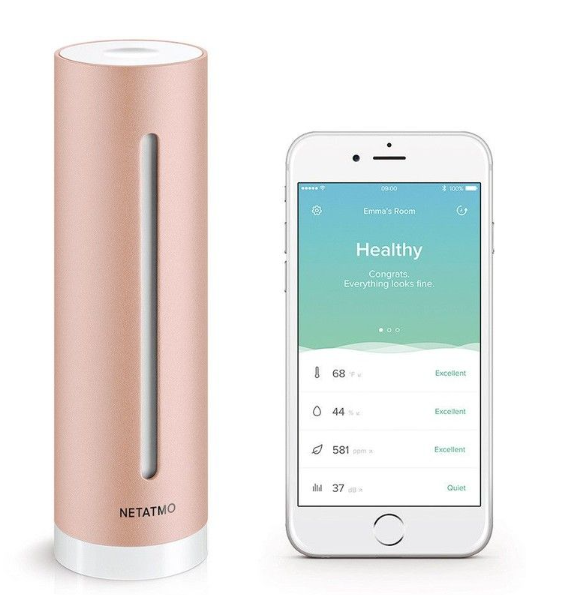
\includegraphics[width=0.4\textwidth]{figures/Netatmo.png}
    \caption{Netatmo Smart Indoor Air Quality Monitor and corresponding app Healthy Home Coach \cite{NetatmoDevice}}
    \label{fig:Netatmo}
\end{figure}

The Netatmo Smart Indoor Air Quality Monitor sends notifications to the users application when the device sense high temperature, \(CO_2\), humidity or noise and low temperature or humidity. These are default enabled, but can be turned off by the user. The values cannot be changed, but are stated by Netatmo in the app. The unit displays live readings to the user through the app, together with a graphical view of values over a longer period of time. When first installed, the device needs at least 7 days to finish calibrating and read the environment values correctly. 

\subsection{Mill Sense Air Quality Monitor}
Mill Sense Air Quality Monitor measures the indoor air quality with 4 different sensors: humidity, \gls{TVOC}, temperature and \(eCO_2\) \cite{Mill}. The monitor communicates to the user's mobile phone through WiFi and connects its data to their own app called \textit{Mill Norway}. It is possible to use Mill Sense together with other Mill units, such as heaters or air purifiers,  to change their values based on the sensor data from Mill Sense \cite{Mill}. 

Figure \ref{fig:MillSenseBoth} shows Mill Sense and its corresponding application, Mill Norway. 

\begin{figure} [H]
    \centering
    \begin{subfigure}{0.3\textwidth}
         \centering
         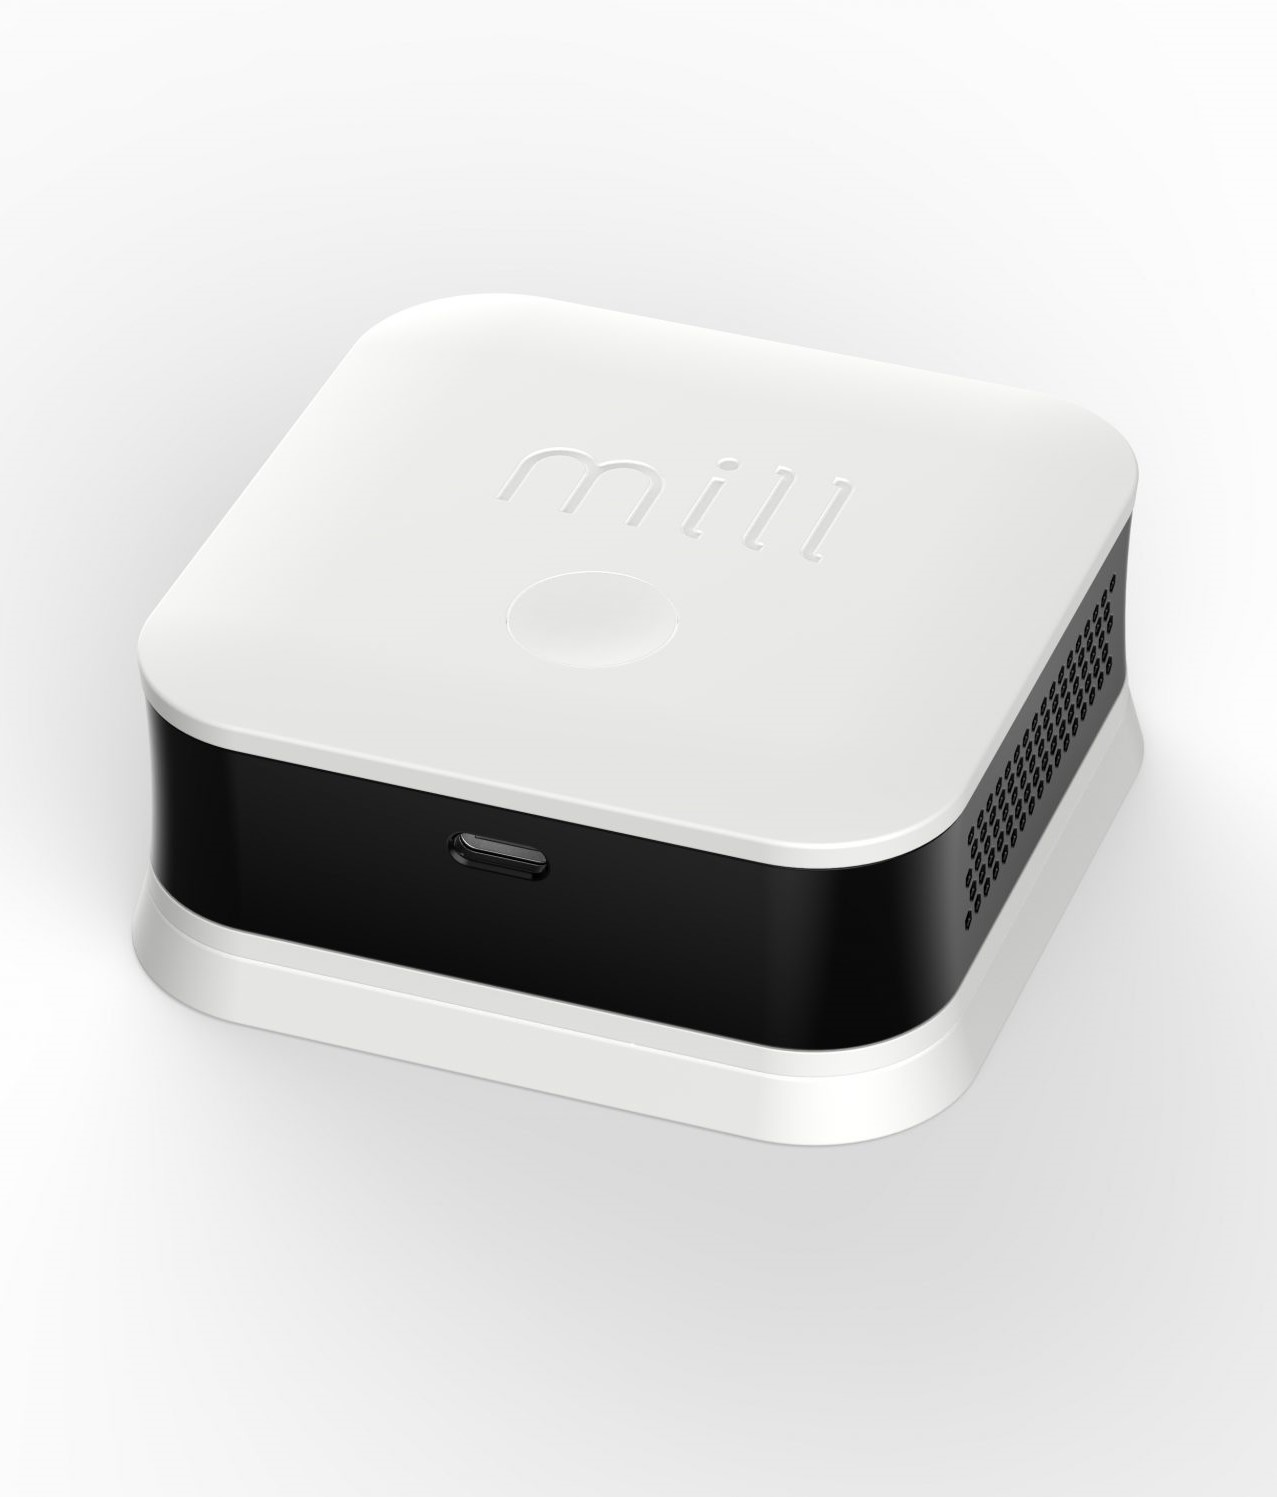
\includegraphics[width=1\textwidth]{figures/MillSense.jpg}
         \caption{Mill Sense device \cite{MillSense}}
         \label{fig:MillSenseDev}
     \end{subfigure}
     \hspace{2cm}
    \begin{subfigure}{0.3\textwidth}
         \centering
         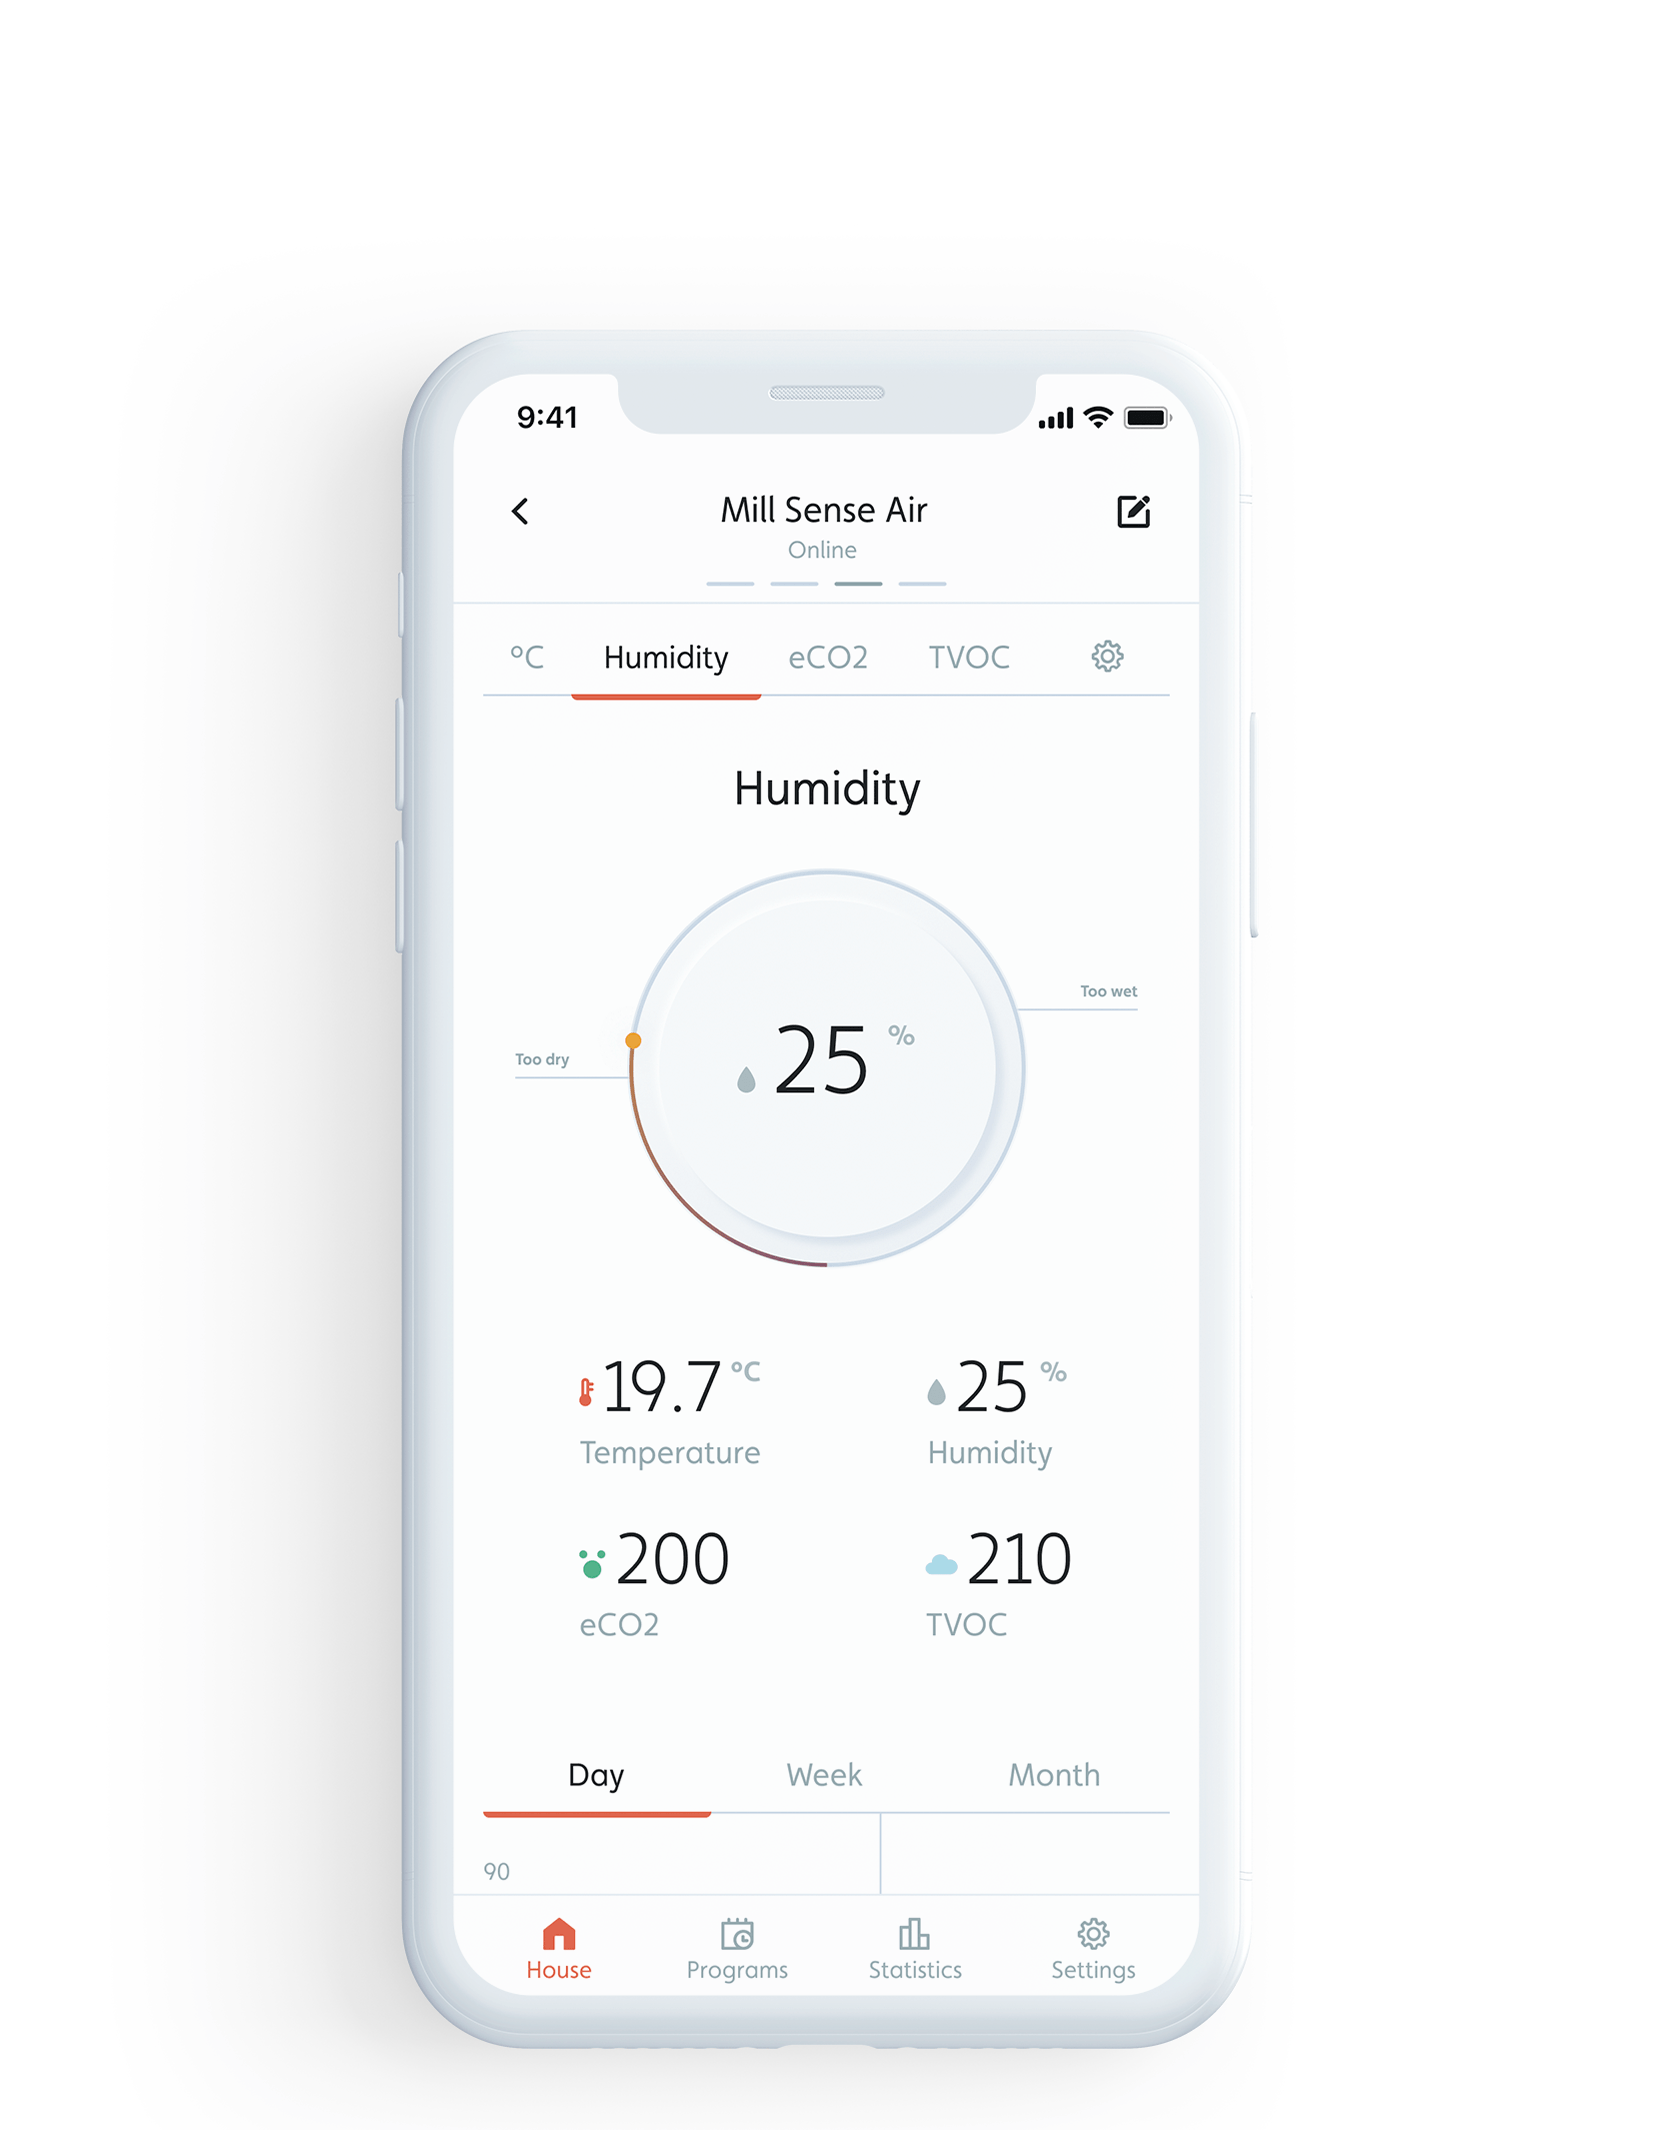
\includegraphics[width=1\textwidth]{figures/MillSenseApp.png}
         \caption{Mill Norway \cite{MillSense}}
         \label{fig:MillSenseApp}
     \end{subfigure}
     \hfill
        \caption{Mill Sense and corresponding app Mill Norway}
        \label{fig:MillSenseBoth}
\end{figure}

The \gls{AQM} does not need power to stay connected and can be placed in any preferred room. The app does not provide notifications to users of threshold levels, but displays the current levels in the app together with graphs that shows variations back in time. Instead of sending notifications to a users phone, the device shows different light responses on the physical unit. These threshold values can be customized. The sensor data collected from the environment is sent to the cloud and back to the users app. It is possible to choose at what time interval the device will send sensor data, from every minute to every hour. When the unit is turned on for the first time and installed in the environment, the device needs at least 5 days to calibrate its sensors. 

\subsection{Nedis SmartLife Air Quality Monitor}
Nedis SmartLife Air Quality monitor has 3 different indoor \gls{AQM} sensors: humidity, temperature and VOC \cite{NedisDevice}. The monitor communicates over \gls{Wi-Fi} to the app, Nedis SmartLife. As Nedis sells several other smart devices, the unit can be integrated in a smart environment together with other devices. 

Figure \ref{fig:NedisBoth} shows Nedis SmartLife Air Quality Monitor and its corresponding application, Nedis SmartLife. 
\begin{figure} [H]
    \centering
    \begin{subfigure}{0.35\textwidth}
         \centering
         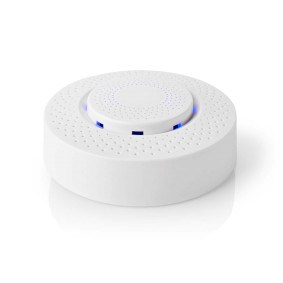
\includegraphics[width=1.2\textwidth]{figures/NedisDevice.jpg}
         \caption{Nedis SmartLife Air Quality Monitor \cite{Nedis}}
         \label{fig:NedisApp}
     \end{subfigure}
     \hspace{2cm}
      \begin{subfigure}{0.35\textwidth}
         \centering
         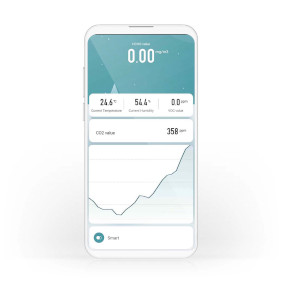
\includegraphics[width=1.2\textwidth]{figures/NedisApp.jpg}
         \caption{Nedis SmartLife App \cite{Nedis}}
         \label{fig:NedisDev}
     \end{subfigure}
     \caption{Nedis SmartLife and corresponding app Nedis SmartLife}
     \label{fig:NedisBoth}
\end{figure}

Nedis SmartLife does not have notifications enabled default, but it can easily be set and customized by the user. Every sensor reading from the device can be set to notify whether levels are too high or too low. The readings on the app shows live data as well as a graphical view of previous readings up to a year before. For setup and calibration in an environment, Nedis does not specify any calibration time.  

\section{Method Tree}
This research is structured in six different main activities, shown in Figure \ref{fig:MethodTree}:

\begin{figure} [H]
    \centering
    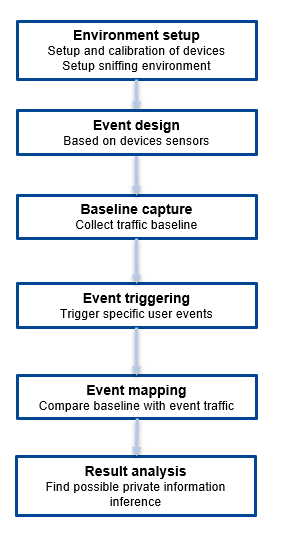
\includegraphics[width=0.5\textwidth]{figures/MethodTree.png}
    \caption{Method Tree}
    \label{fig:MethodTree}
\end{figure}
\subsection{Environment Setup}
The first main activity is to set up the environment with both hardware and software correctly configured. The air quality monitors, the sniffer, the hardware and software are explained in this Subsection. 
\\
\textbf{Air Quality Monitors}\\
The \gls{AQM}s needs to be installed, connected to the app and calibrated. The devices were installed and connected to the app as explained in the user manual attached to the devices. They were all installed in the smart home environment for a longer period than their required for calibration. It is desirable that the air quality monitors gives notifications when a certain threshold value is met. However, for Mill Sense it is not possible to set notifications, but Nedis SmartLife and Netatmo Smart Indoor Air Quality Monitor were set with the same threshold values for notifications. The \gls{MAC} addresses for the air quality monitors can all be found in their corresponding apps, since identifying and discovering the devices are out of scope for this thesis. 

Table \ref{tab:AQMSetup} describes each \gls{AQM}, their \gls{MAC} address and which sensor values triggers the devices to send notifications to the users phone. For the rest of this thesis, the devices will only be referenced with their manufactures name; Netatmo, Mill and Nedis, to simplify the presentations. 
 
\begin{table}[H]
    \centering
    \caption{\gls{MAC}-address and notification threshold values for each \gls{AQM}}
    \begin{tabular}{| p{3.5cm} | p{3.5cm} | p{5cm} |} 
        \hline
        \textbf{Air Quality Monitor} & \textbf{\gls{MAC} Address} & \textbf{Notification threshold values} \\
        \hline
        Netatmo & 70:EE:50:91:06:DE & \(CO_2\) > 1150 ppm \newline Noise > 62db \newline Humidity < 30\% \newline Humidity > 60\% \newline Temperature < 17 \degree C \newline Temperature > 26 \degree C \\
        \hline
        Mill & B8:F0:09:B3:B3:78 & None \\
        \hline
        Nedis & 2C:F4:32:29:36:DC & \(CO_2\) > 1000 ppm \newline Humidity < 30\%  \newline Humidity < 50\% \newline Temperature < 15 \degree C \newline Temperature > 25 \degree C \newline VOC > 99.9 ppm\\
        \hline
    \end{tabular}
    \label{tab:AQMSetup}
\end{table}

\noindent
\textbf{Sniffer}\\
In order to collect all \gls{Wi-Fi} traffic within the environment, a network sniffer needs to be configured. The sniffer needs to be able to connect to the system were the packet capturing will take place and be set in monitoring mode. It exists a wide variety of available \gls{Wi-Fi} sniffers online, but selected sniffer in this research is the TP-Link TL-WN722N. 

\begin{figure} [H]
    \centering
    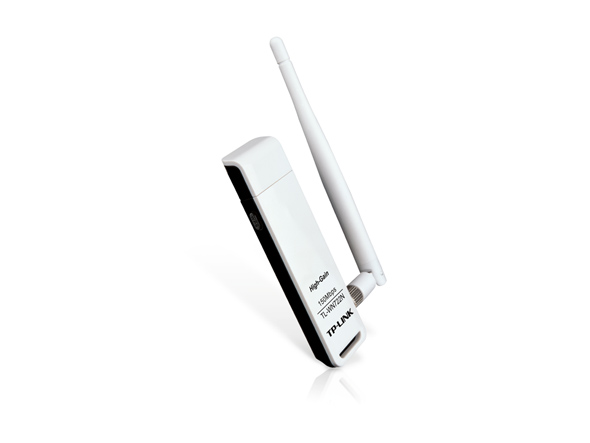
\includegraphics[width=0.5\textwidth]{figures/Sniffer.jpg}
    \caption{The \gls{Wi-Fi} sniffer selected in this research: TP-Link TL-WN722N \cite{Sniffer}}
    \label{fig:Sniffer}
\end{figure}

To set the device in monitoring mode, the sniffer first plugged into a computer, raspberry pie or similar and then the following four commands were applied on the sniffer:

\begin{verbatim}
    sudo ifconfig wlan0 down
    sudo iwconfig wlan0 mode monitor
    sudo ifconfig wlan0 up
    sudo iwconfig
\end{verbatim}

Note that Wlan0 was the assigned wlan for the device when it was plugged it into the environment, so it needs to be changed to monitoring mode accordingly. The specific wlan addressed to the sniffer can vary from system to system so it needs to be checked with the device is plugged into the system. When the sniffer is configured in monitoring mode, the device are able to collect all \gls{Wi-Fi} traffic that is within its own signal range. In this way, the sniffer will be able to collect the traffic sent to and from the \gls{AQM}s installed in the environment. To verify that the sniffer is collecting traffic on the network, Wireshark were used with the corresponding wlan, Wlan0, as capturing interface. 

\textbf{Tshark}\\
In order to store and process the traffic that the TP-link collects, a monitoring software was used. Tshark \cite{Tshark} is an open and free network packet analyzer and will be used to store packets. Tshark can be run from the command line interface and has the possibility of using capture filters based on a number of parameters, such as addresses, duration or size. In order to store the packets captured, tshark was run with the option of writing its results to an output file rather than directly in the command-line, as it does in default. The packets collected in the output file by tshark are possible to open and analyze in Wireshark. 

To store packets from all the three air quality monitors, tshark was run from three different terminals with corresponding filter as the devices. The options of the command are explained in Table \ref{tab:tshark}.

\begin{table}[H]
    \centering
    \caption{Tshark command options used to capture traffic}
    \begin{tabular}{|l|l|}
    \hline
    \textbf{Filter option} & \textbf{Usage}                        \\ \hline
    tshark                 & Initialize tshark                     \\ \hline
    -i                     & Interface to be used                  \\ \hline
    -f                     & Capturing filter                      \\ \hline
    -w                     & Output file to store captured packets \\ \hline
    \end{tabular}
    \label{tab:tshark}
\end{table}

\newpage
\begin{verbatim}
Netatmo:
    tshark -i wlan0 -f ether.host == 70:EE:50:91:06:DE -w 
    \\Documents\Netatmo
Mill:
    tshark -i wlan0 -f ether.host == B8:F0:09:B3:B3:78 -w 
    \\Documents\Mill
Nedis:
    tshark -i wlan0 -f ether.host == 2C:F4:32:29:36:DC -w 
    \\Documents\Nedis
\end{verbatim}

\noindent
\textbf{Platform}\\
To collect data and store it from the devices, an operating system running on a hardware component with the possibility to connect the sniffer were setup. In this thesis, a Raspberry Pi Model 3 B+ were chosen as it can continuously be powered on to capture traffic over longer periods of time. The Raspberry Pi was installed with Kali Linux version 2022.3, which can be installed from \cite{KaliLinux}, which was beneficial as it includes all the needed software to capture the traffic and it is compatible with the TP-link sniffer. As the analysis will be conducted on another computer, WinSCP were used to download the files from the Raspberry Pi over the network, which can be downloaded from \cite{WinSCP}. Figure \ref{fig:Environment} shows a logical overview of the setup of the environment.  

\begin{figure} [H]
    \centering
    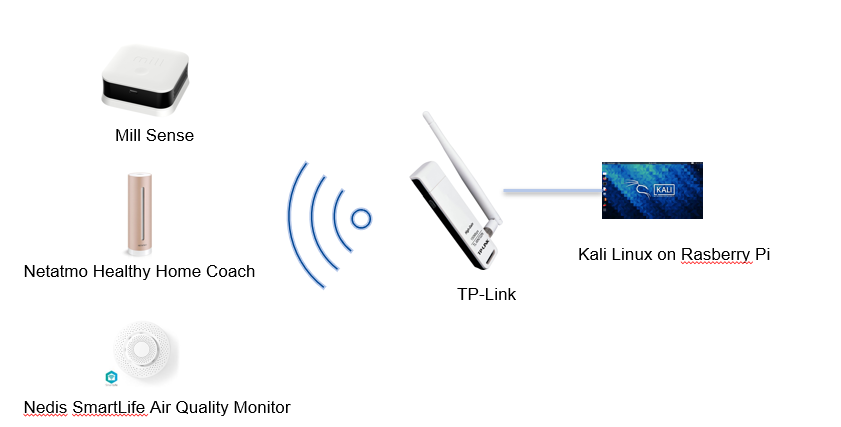
\includegraphics[width=1\textwidth]{figures/Environment.png}
    \caption{\gls{Wi-Fi}: Environment setup with all devices \cite{MillSense}, \cite{NetatmoDevice}, \cite{NedisDevice}}
    \label{fig:Environment}
\end{figure}

\subsection{Event Design}
\textbf{Justification of test cases}\\\\
In order to infer user behaviour from the devices, several test cases were designed. As the \gls{AQM}s are installed and monitors the home environment at all times, the test cases are not limited in time or place in the house as they can be moved. The traffic characteristics are unknown, and therefore a hypothesis tree can be used to better understand how to proceed based on the results from the traffic analysis. 

Figure \ref{fig:HypothesisTree} shows the hypothesis tree of this research:

\begin{figure} [H]
    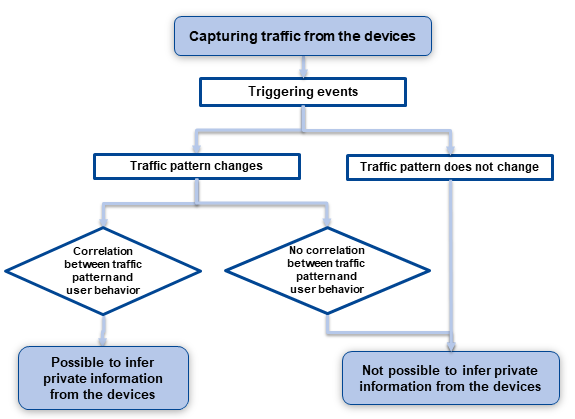
\includegraphics[width=1\textwidth]{figures/Hypothesistree.png}
    \caption{Hypothesis Tree}
    \label{fig:HypothesisTree}
\end{figure}

Looking at the different sensors and how they can be affected is important for understanding which user behaviour can possibly change traffic pattern. All the sensors from all the devices are; \(eCO_2\), \(CO_2\), humidity, temperature, \gls{TVOC}, \gls{VOC}, HCHO and noise. Some of the sensors will be affected by the same actions, so they will be categorized together. The following significantly different categorized sensors will be used: \(CO_2\), humidity, temperature, VOC and noise. 

Examples of user behaviour in a home that affects the different sensors:
\begin{itemize}
    \item $\mathbf{CO_2:}$ People or animals present, cooking, windows open
    \item \textbf{Humidity:} Windows open, showering
    \item \textbf{Temperature:} People or animals present, windows open, fireplace lit
    \item \textbf{VOC:} Cooking, burning candles
    \item \textbf{Noise:} Many people present, playing music or TV
\end{itemize}

Several of the proposed user behaviours will affect not only one, but several sensors. However, it is more beneficial to focus on routines that users do every day to be able to see a pattern of a household instead of looking at one specific action that users may not do regularly. It is also important to notice that in order to infer private information from network traffic, the test cases needs to change the sensor values by some degree. So even though people and animals present is an interesting private information to infer, this will not affect the thresholds enough in a routine way. Therefore, repetitive behaviour that has the possibility to change the threshold values are chosen. 

The three different routinely test cases chosen are \textbf{cooking}, \textbf{showering} and \textbf{windows open at night}. Cooking is the most routinely behaviour in a home where dinner is normally made every day. The next test case is showering as this is a routine behaviour and will affect the sensors, particularly humidity and temperature in the bathroom. Showering can be routinely done at very different times, but evening showers are used in this case. Windows in a home can be open at several times, however, having a window open every night while sleeping can be common for many and should drastically change the indoor temperature and possibly humidity. Especially since the testing will be carried out during winter time in Norway. This is also a test that will last longer than the other two tests and can possibly give another aspect to the research. 

Another test case that can be interesting to see if changes the traffic patterns of the data sent to and from the \gls{AQM}s is when the user are home or not. To be able to test this, a weekend test will be carried out. The sniffer will gather traffic from several weekends when the user is present in their home environment and compare it to when the user is away for the weekend and look at the differences. If it is possible to infer whether a user is home or not by looking at the traffic patterns, an adversary can misuse this private information. 

\subsection{Baseline Capture}
To be able to distinguish the events in the \gls{Wi-Fi} traffic, it is necessary to capture and analyze traffic from the devices when they are not affected by any events. This is necessary to understand what normal traffic from the devices are. During a baseline capture, the devices were installed and calibrated in the environment. All notifications that will be enabled during the event triggering are enabled. The devices were reachable through their app and communicate in their own pattern. The baseline capture was on-going for several days to ensure enough data and traffic was collected. During this capture, the devices were placed in the inner hallway of the apartment. It would have been ideally to have a baseline from each room of where the test cases will be located, but due to time constraints, they were placed in a room binding all the other rooms together. 

\subsection{Event Triggering}
In this activity, traffic from the devices were captured while the events triggered. The routine events are each triggered 10 times and traffic from at least 1 hour before and after the event are captured to see the changes in traffic both before and after the events. Weekend testing were conducted in the course of 14 weekends, resulting in collected traffic from 7 weekends at home and 7 weekends away. 

Table \ref{tab:TestCases} gives an overview of the time of day when each test case was carried out and in which room the devices were placed for the tests. 
\begin{table}[H]
    \centering
    \caption{Overview of test cases with timings and location}
    \begin{adjustbox}{width=1\textwidth}
    \begin{tabular}{| p{5cm} | p{5cm} | p{3cm} |} 
        \hline
        \textbf{Test Case} & \textbf{Time of day} & \textbf{Room} \\
        \hline
        Cooking & After work: 4pm to 5pm & Kitchen \\
        \hline
        Window open at night & At night: 11pm to 7am & Bedroom\\
        \hline
        Showering & Afternoon: 8pm to 9pm & Bathroom \\
        \hline
        Weekend tests & Friday: 4pm to Sunday: 11pm & Living room \\
        \hline
    \end{tabular}
    \end{adjustbox}
    \label{tab:TestCases}
\end{table}

As there is only one of each device and the tests are in different rooms, the devices will be moved to the corresponding room before each test. The devices will be placed in the environment for at least 1 hour before each test starts to ensure that the value changes between the room will be as equalized as possible. The exact times for when cooking, open window and showering took place were be logged so it is possible to look for changes at that time. 

Figure \ref{fig:Apartment} shows an overview of the apartment layout, hereby called \textbf{the environment}, where the test cases and baseline will be captured from. The different rooms are marked and shows where the devices will be placed during the different tests. 

\begin{figure}[H]
    \centering
    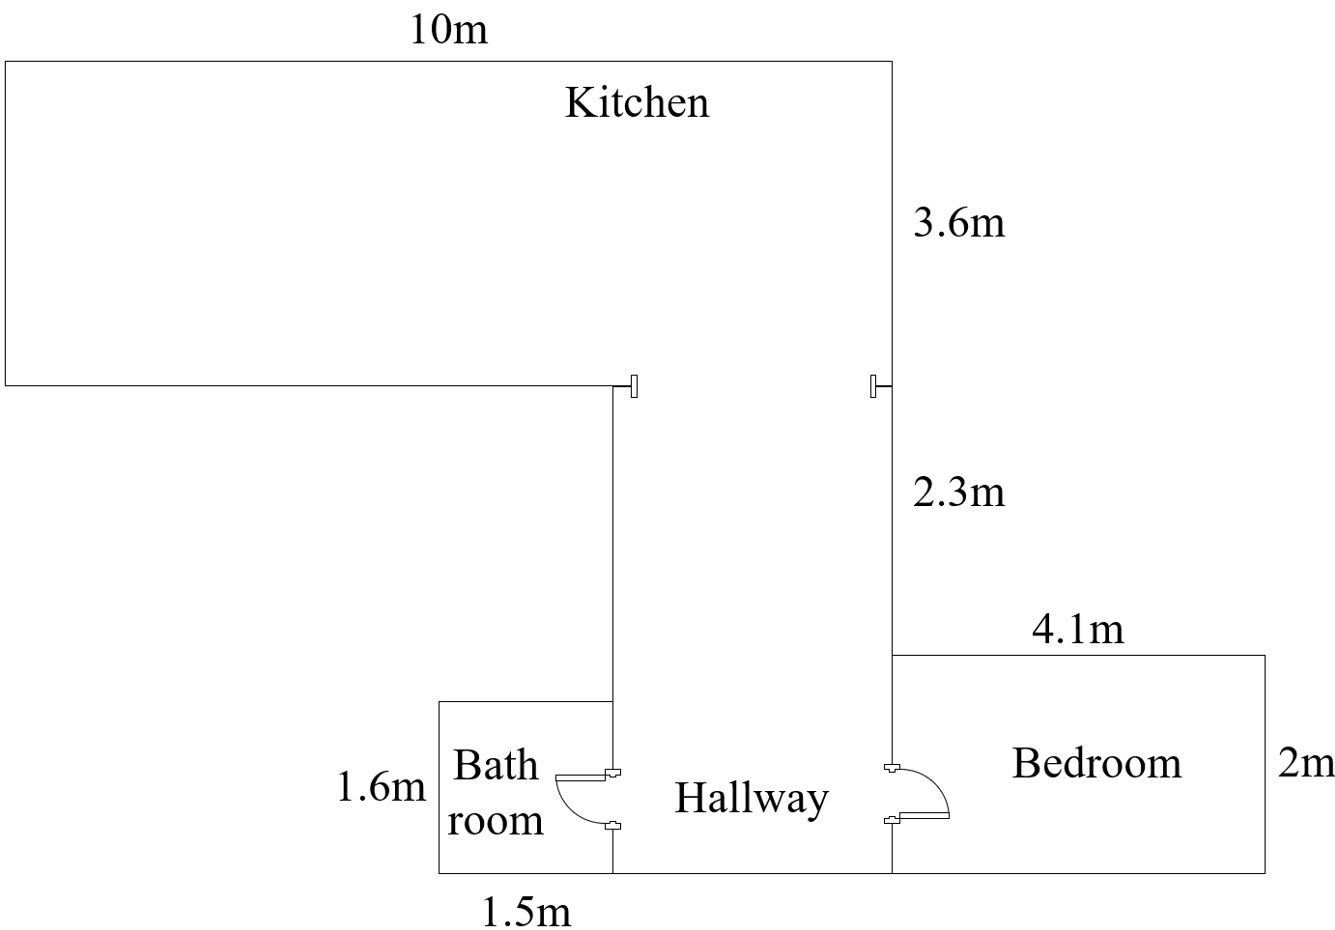
\includegraphics[width=0.7\textwidth]{figures/Apartment.png}
    \caption{Overview of the environment for the test cases and baseline capturing. Cooking in the kitchen, showering in the bathroom, window open at night in the bedroom and baseline in the hallway.}
    \label{fig:Apartment}
\end{figure}

\subsection{Event Mapping}
When the events have been carried out, a mapping was made to see if information could be inferred. Each event are presented both graphically and numerically with different calculations to be able to compare. Each event were extracted from the corresponding tshark capture saved in the pcap file. A separate pcap file for each event were made, with the timing of the specific event to see differences. 

\subsection{Result Analysis}
The last activity is to analyze the results from the tests performed. For each event; cooking, showering, window open and weekend, several graphs and calculations are presented side by side to be able to analyze. This is divided into categories with the three different devices. Then the actual events are compared to the baseline for each device to look further into mapping the events from standard traffic. The results are commented and evaluated in the same sections that presents the results, and a separate subsection is presented to discuss and answer the research questions presented in Chapter 1. 
\chapter*{Evaluation and Analysis Results}
\section*{Specifications}
\section*{Environment}
\section*{Test cases}

\chapter{Discussion}
This chapter discusses the research questions by using the results found in the four test cases of this research. The questions will be answered sequentially. The chapter also discusses the work done in this thesis, both what was done good which lead to new knowledge and contributions, but also what could have been done differently. Challenges and mistakes which lead to decisions being made are explained here. Limitations to this research will also be included as this could have affected how strong the results are and can explain why certain decisions were made. 
\section{Answer to the research questions}
As presented in Chapter 1, the research questions to be answered in this thesis are:

\begin{enumerate}
    \item What kind of information can be gathered from air quality monitors when carrying out a passive network eavesdropping attack?
    \item What are the differences in level of inference from different air quality monitors from different vendors?
    \item How can the private information gathered be misused by an adversary?
\end{enumerate}

In this research, four different test cases have been used to test if it is possible see traffic pattern changes from when an event is triggered in the environment the device relies. By looking at calculations and graphical views over the traffic flows during the test, we were able to find results to answer the research questions in this thesis. The baseline capturings showed that all the devices communicates with a layer of security, as the packets sent on \gls{Wi-Fi} is encrypted and not readable while carrying out a passive network eavesdropping attack. Therefore it is not possible to gather private information sent in the payloads to and from the devices. 

For the routine behavioural events defined as cooking, showering and window open, only showering and window open gave notifications of threshold values exceeded for all executions. None of the devices showed a significant difference from when an event was triggered at a specific time compared to the traffic sent before and after the event or compared to the baseline capturings. While comparing the baseline traffic to the event traffic, the devices Nedis SmartLife and Mill Sense showed that there are visible differences from the baseline capturings to right before and after the events which should expectedly have been the same. This can be a result that the traffic can be affected by smaller indoor changes such as a season can change the indoor air quality. For example, during summer windows can be more open than during winter were ovens can be more used. 

However, for the weekend test, one of the devices shows a clear difference from when a user is home or gone during the time period of a weekend. When Netatmo Smart Indoor Air Quality Monitor was used, it shows that it is possible to distinguish whether a user is home or gone by looking at the total number of bytes sent and received to that device during the weekend and looking at size of the packets sent by the device which is never higher than 134 bytes when the user is gone for the weekend. This kind of information will expose private information about a user were it is possible to see whether the user is home or not for a longer period of time. These two factors proves that it is possible to infer private information form the device. For Mill Sense and Nedis SmartLife, no similar findings were discovered during the tests. 

In the weekend testing, it looked like there were differences for both Mill and Netatmo for the first 5 weekends at home, but only Netatmo had the same significantly different pattern for weekends at home and gone. For Mill, the pattern changed for the two last weekends at home where the packet size were the same as for the weekends gone. This shows the importance of including enough executions for each of the test cases. However, for over 70\% of the weekends at home, a clear difference is visible when a user is at home compared to gone. Due to time constraints, no more weekends were tested, but more tests could reveal if these two weekends were an exception or if it is not possible to distinguish a weekend at home or gone for this device. For Nedis, no significant differences were possible to see during the weekend testing and therefore private information about whether a user is at home or gone during the weekend was not possible to discover during these tests. 

The baseline capturings shows that the devices communicates differently. For Netatmo and Nedis, most of the packets are outbound bytes meaning that these devices send a lot more traffic than they receive. For Mill, inbound traffic was higher than outbound traffic. Also comparing the traffic from the three devices, as shown in Figure \ref{fig:ComparingBaselines}, shows that the traffic is different from the three devices. Netatmo has a more continuous line of the packets, while Mill sends traffic periodically and have more spikes and Nedis shows many spikes that are a lot higher than for the rest of the baseline period. These differences can be used to distinguish the traffic between the three air quality monitor from different vendors. 

The differences in level of inference from the three different air quality monitors are only distinguishable when it comes to Test Case 4: Weekends. For the routine behavioural test cases, neither of the devices expose private information regarding when the event is ongoing or what kind of event is triggered. However, the results from the weekend test shows that Nedis and Mill is a more secure choice than Netatmo when it comes to selecting air quality monitor to install in our home. Also when it comes to identifying changes in traffic, Nedis and Mill shows that the baseline traffic can change on other factors than a triggered event and it will therefore be harder for an attacker to understand normal traffic. It is good for users to know that one should consider more factors than just the appearance or functionality of the air quality monitor when selecting what device to install in their home. Knowing that the network traffic of an air quality monitor is not the same regardless of the manufacture, is important when selecting the right one. 

As only the weekend test for Netatmo exposed private information, only this specific test case can be used to evaluate how this information can be misused by an adversary. If an adversary has conducted a passive network eavesdropping attack against a user who has installed the Netatmo Smart Indoor Air Quality Monitor, it is possible to know if a user is gone for a longer period of time. Even though weekends were used in this test, the results will also be applicable for longer periods of time such as a week or several weeks. An adversary could use this private information to carry out malicious actions against the users home such as a burglary. Another aspect is that an attacker could learn about our habits for being home or not, such as every Easter or Christmas, the user is gone or every weekend during winter the user is not home. 

However, it is interesting to consider to what extent private information from the other test cases can be misused. Both cooking and showering are events where the users is awake and doing an active action in the home environment. If an adversary were to find out the routines of a user for these two cases, it may not be able to misuse it to the extent as the results from the weekend test can. Knowing that an unwanted party knows that every day at 7am you are taking a shower, may not feel that scary and invading, but if this is combined with attacks against other devices to find out your whole daily routine, it can feel like a bigger invasion of privacy. Window open at night can indicate a users sleeping patterns and therefore identifies a time period where the user is not awake in its home environment. This can feel like a more invasion of privacy as the user does not have as much control over the situation as when cooking or showering. On the other side, being able to know if a user is gone for a whole weekend is easier to misuse than just sleeping as the user is present at home.   

\section{Valuable contributions and challenges faced}
When starting this research, a decision to include several different air quality monitors from different manufactures were made. Looking at the results and evaluation, this was positive for the contribution as it shows that there are differences in level of private information inference from the different devices. This shows that analyzing the network traffic from one air quality monitor is not representative for all air quality monitors and is something to consider if setting up a test environment where only one air quality monitor is included.

Originally, only the routine test cases were selected, cooking, showering and window open. For the work of setting up the devices, sniffer and how to capture, traffic was captured over a longer period of time to also test the storage and processing power of the hardware used. During this initial setup, a discovery of the differences in traffic for Netatmo Smart Indoor Air Quality Monitor from when the user was gone or not were very visible. Therefore, the fourth test case was defined and tested on all the devices. 

When defining the scope and test cases, it was unclear how the devices communicated including packet sizes, amount of packets, how frequent and if traffic was encrypted or not. When starting the capturing and analyzing of data from the different devices, it became clear that the devices do not send the same amount of traffic. Netatmo Smart Indoor Air Quality Monitor sends the least amount of packets, while Mill Sense and Nedis SmartLife sends significantly more packets. For Nedis SmartLife, analyzing the amount of traffic was a challenge, both time-wise as creating graphs took a long time, but also looking more into the traffic. The processing power of a standard computer were just enough to process the data and figures shown in the evaluation and analysis result chapter. 

Many decisions and limitations had to be set for this research because of time constraints. Originally the plan was to test more air quality monitors from other manufactures, communicating on different communication protocols, such as Bluetooth or ZigBee. However, seeing the amount of work and results that needed to be analyzed to do this in a good way, only \gls{Wi-Fi} devices were selected. This part is therefore moved to future work.  

A challenge faced during the research happened for the test cases for cooking. The events were designed to change the indoor environment so much that the air quality monitors would sense values outside of the defined threshold values. However, when doing the cooking test, only a few of the executions actually triggered the notifications to be send. On the other side, for showering and window open, every execution lead to a significant change in threshold values and sent several notifications to the connected phone. 

Another challenge encountered during the test, was the differences in the baseline capturings compared to the event traffic for Nedis SmartLife and Mill Sense, before the event was triggered, as we would have expected these two traffic patterns to be similar. However, the decision were made to include the baseline capturings and compare them to the event traffic because it also shows methodologically the setup that was originally designed, and it is still possible to compare traffic from when the event was ongoing to traffic before and after the event. It is unclear why there are differences in standard traffic from the devices, but differences in season as the test cases have been conducted during January and the baseline during March can be one reason. Another reason can be that the baseline was not captured at the exact same spot as were the test cases were carried out. This was because of time constraints. It was not enough time to have a long baseline in each room and conduct the test cases during the research period even though this would have been preferred. Since the air quality monitors are \gls{IoT} sensor that are always on and sense the environment at the time, differences day to day and month to month can be significant. The indoor environment can be affected by many different factors and it is impossible to have the exact same values for the indoor air during longer period of times. 

The differences in standard traffic shows that in order to have the same traffic pattern to test with, the best way would be to have the air quality monitors in a closed environment. Then the environment could only be changed by the specific event which are tested. However, this takes away the realistic parts of the test. The chance of identifying the specific events may be bigger, but if it is not applicable in a live environment, there is no use to launch such an attack against a target. Another aspect of this is that if changes in the environment is significant within the same environment then it will also be hard for an attacker to find certain signatures in their own environment to be applicable on a target environment and device. 
\chapter{Conclusions and Future Work}
This thesis has investigated three different air quality monitors to see what kind of private information can be inferred while carrying out a passive network eavesdropping attack. Three research questions have been raised and answered through the tests in this thesis. The three devices selected were Netatmo Smart Indoor Air Quality Monitor, Mill Sense and Nedis SmartLife. To test which kind of private information can be inferred from the devices, the devices were installed in a live environment and four different test cases were carried out. Three test cases which targets routine behaviour; cooking, showering and window open during night, and one test case over a longer period of time; home or gone during a weekend. 

The initial baseline capturings for each device showed that the devices communicates quite differently in number of packets and bytes sent and received and packet sizes. Scripts for generating graphs of the traffic flows in a presentable way were created and used to present the results. The three routine test were compared with corresponding times for baseline capturings. For Mill Sense and Nedis SmartLife, the baseline traffic differs from the same standard traffic that is captured before an event is triggered. This shows how the network patterns of these devices can be affected by factors such as season or location. For Netatmo Smart Indoor Air Quality Monitor, the baseline traffic is comparable to the event traffic. 

The routine tests were carried out over 10 different days to have enough capturings to look for a specific traffic pattern. During these tests, only showering and window open during night triggered the sensor thresholds as expected and sent notifications to the application. For cooking, not every execution did this. When looking at the traffic patterns for these test cases and devices, there are no significant change in traffic pattern from before an event is triggered to when the event is ongoing. This applies to the three test cases cooking, showering and window open for the three devices Netatmo Smart Indoor Air Quality Monitor, Mill Sense and Nedis SmartLife.  

The weekend tests were carried out over 14 different weekends with 7 of them at home and 7 gone. For the weekend test, Mill Sense and Nedis SmartLife did not expose differences in traffic patterns from when a user was home or gone. However, for Netatmo Smart Indoor Air Quality Monitor the results shows a clear difference. When a user is home, the device sends significantly more bytes and bigger packets compared to when the user is gone. This information can be misused by an adversary to know if a user is home during a weekend or a holiday and perform malicious actions such as burglary. 

Through carrying out four test cases on three different air quality monitors, the research questions have been answered. Only one of the devices exposed private information in one of the tests and shows that using this method, the majority of private information tested are not revealed. However, Netatmo reveals private information whether a users is home or not for longer periods of time by looking at the traffic patterns on \gls{Wi-Fi} traffic. This research shows that different air quality monitors communicate with different network patterns on \gls{Wi-Fi}. It is therefore important to understand that the choice of air quality monitor can impact how much private information it is possible to infer. This is applicable both in research cases and when choosing an air quality monitor to install in a home environment. The scripts created to generate graphs of traffic flows and methods used can be used to further test other air quality monitors also communicating on other communication protocols.
\\\\
\textbf{Future Work}
\\
This research is limited to investigating air quality monitors which communicates over \gls{Wi-Fi}, therefore future researches could look into differences between communication protocols and include air quality monitors that communicates over protocols such as Bluetooth, ZigBee or Z-wave. Since Netatmo Smart Indoor Air Quality Monitor reveals private information during the weekend-testing, building further on these findings could be to look into timings for when the traffic pattern changes. This research only showed during a weekend or longer gone, but testing for days or hours could also give more information as to how easy it is to see when a user is home or not. Another aspect is testing the devices in an environment with other \gls{IoT} devices to see if there are differences in test cases or if it reveals more or less private information than other \gls{IoT} devices. This thesis does not look into security measurements, but as one of the tests discovers private information on the target environment, future work should look into how implement security measurements to this case. 



\chapter*{\bibname}
\printbibliography[heading=none]

\appendix
\renewcommand{\thesection}{\Alph{section}}
\appendixpage
\section{Script to generate graphs for baseline comparison with packets as reference}
    \lstinputlisting[language=python, breaklines=true]{appendices/GraphsByPackets_BaselineEvents.py}
    \label{app:GraphsByBytes}
\newpage
\section{Script to generate graphs for baseline comparison with packets as reference}
    \lstinputlisting[language=python, breaklines=true]{appendices/GraphsByPackets_BaselineEvents.py}
    \label{app:GraphsByPackets}
\newpage
\section{Script to generate graphs for baseline comparison with packets as reference}
    \lstinputlisting[language=python, breaklines=true]{appendices/GraphsByPackets_BaselineEvents.py}
    \label{app:GraphsByBytes_BaselineEvents}
\newpage
\section{Script to generate graphs for baseline comparison with packets as reference}
    \lstinputlisting[language=python, breaklines=true]{appendices/GraphsByPackets_BaselineEvents.py}
    \label{app:GraphsByPackets_BaselineEvents}
\end{document}